\section{Exercise 02}
\subsection{}

\begin{frame}
\frametitleTC{Building a block diagram in Modelica}
\framesubtitleTC{and experimenting with direct synthesis}
\myPause
 \begin{itemize}[<+-| alert@+>]
 \item Launch the model editor OMEdit.
 \item Issue \texttt{File->New Modelica Class}.
 \item Name the class \texttt{PID4CS}, select \texttt{Package} as \texttt{Specialization}. \underline{un}check\\
       \texttt{Save contents in one file} and click \texttt{OK.}
 \item You just created a \texttt{package}, a hierarchically organised collection\\
       of models.\\
 \item Right-click the P (Package) entry \texttt{PID4CS} in the \texttt{Libraries Browser}\\
       on the left, select \texttt{Save As}, and save. A folder named PID4CS\\
       will be created at the location you chose, details on its structure\\
       (inessential here) at \texttt{modelica.org} for the interested.
 \item Right-click \texttt{PID4CS} in the \texttt{Libraries Browser} and select\\
       \texttt{New Modelica Class}.
 \item Create a \texttt{Model} named \texttt{PS02\_ex02}, that will be part of \texttt{PID4CS}.\\
       Expand the entry (small triangle icon on the left) to see.
 \end{itemize}
\end{frame}

\begin{frame}
\frametitleTC{Building a block diagram in Modelica}
\framesubtitleTC{and experimenting with direct synthesis}
\myPause
 \begin{itemize}[<+-| alert@+>]
 \item No more details on the \texttt{Libraries Browser}, it works like any file manager.
 \item Double-click \texttt{PS02\_ex02} to edit: your window should look like
       \begin{center}
        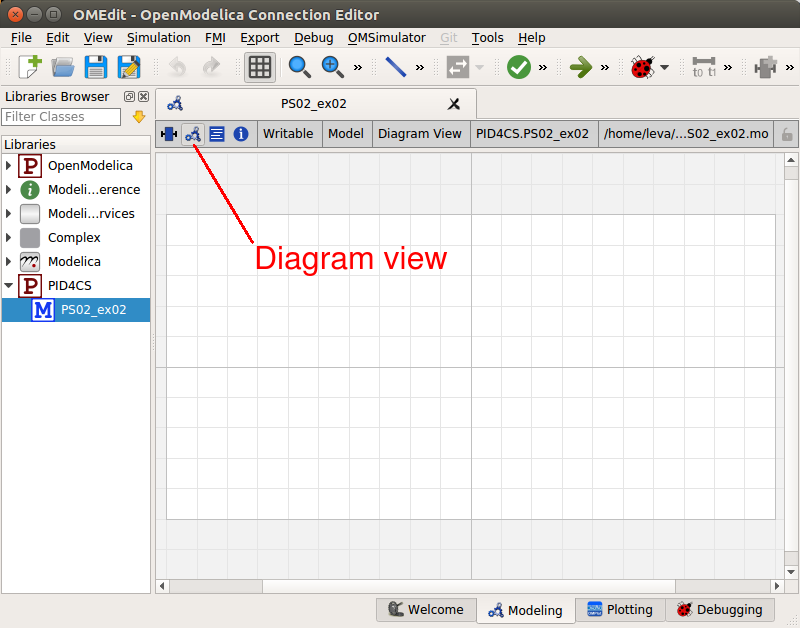
\includegraphics[width=0.40\columnwidth]{./Unit-05/img/PS02-ex02-fig01.png}
       \end{center}
       and you should be in \texttt{Diagram view} (click its button if not).
 \end{itemize}
\end{frame}

\begin{frame}
\frametitleTC{Building a block diagram in Modelica}
\framesubtitleTC{and experimenting with direct synthesis}
\myPause
 \begin{itemize}[<+-| alert@+>]
 \item Open the \texttt{Modelica Standard Library} (MSL for short); it is the \texttt{Modelica}
       entry in the \texttt{Libraries Browser}.
 \item Navigate to the \texttt{Blocks} package, that contains block diagram elements.
 \item You need \texttt{Transfer Function} from the \texttt{Discrete} sub-package, \texttt{Add}
       and \texttt{Feedback} from the \texttt{Math} one, and \texttt{RealExpression} from \texttt{Sources}.
 \item By dragging{\&}dropping from the browser, and wiring by click{\&}drag, create the\\
       diagram below (block types added for your reference, names above blocks):
       \begin{center}
        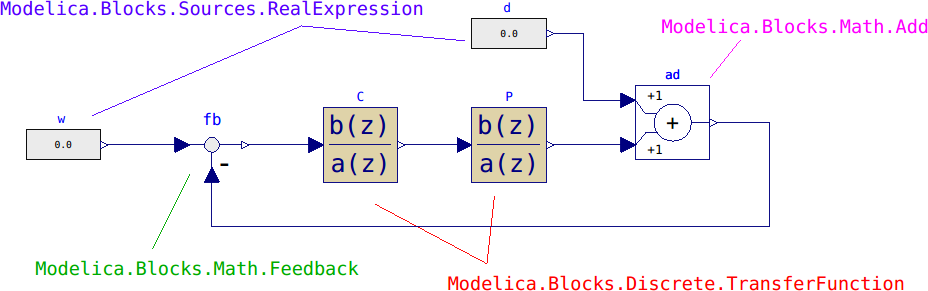
\includegraphics[width=0.60\columnwidth]{./Unit-05/img/PS02-ex02-fig02.png}
       \end{center}
 \end{itemize}
\end{frame}

\begin{frame}
\frametitleTC{Building a block diagram in Modelica}
\framesubtitleTC{and experimenting with direct synthesis}
\myPause
 \begin{itemize}[<+-| alert@+>]
 \item Double-click on the \texttt{P} and \texttt{C} blocks to set their transfer functions. Polynomials\\
       are specified as vectors of coefficient in decreasing power order: for example,\\
       $2z^3+z+5$ becomes \{2,0,1,5\}. Do not forget the braces and the zero entries\\
       for possibly missing powers --- including the constant term, $z$ becomes \{1,0\}.
 \item You also need to set a \texttt{samplePeriod}, i.e., the time between $k$ and $k+1$\\
       (in seconds). For this exercise it is inessential, enter 1 throughout.
 \item Double-click on the \texttt{w} and \texttt{d} blocks to enter the expression of their output\\
       as a function of time (the symbol \texttt{time} is system-declared).\\
       For example, $w=step(k)$ and $d=step(k-10)$ become respectively\\
       \texttt{if time<0 then 0 else 1} and \texttt{if time<10 then 0 else 1}.
 \end{itemize}
\end{frame}

\begin{frame}
\frametitleTC{Building a block diagram in Modelica}
\framesubtitleTC{and experimenting with direct synthesis}
\myPause
 \begin{itemize}[<+-| alert@+>]
 \item Issue \texttt{Simulation->Simulation Setup} to set the final time and then \texttt{Simulate}.
 \item Use the \texttt{Variable Browser} in the \texttt{Plotting} tab to examine the results. Below\\
       is an example with some explanatory lettering.
       \begin{center}
        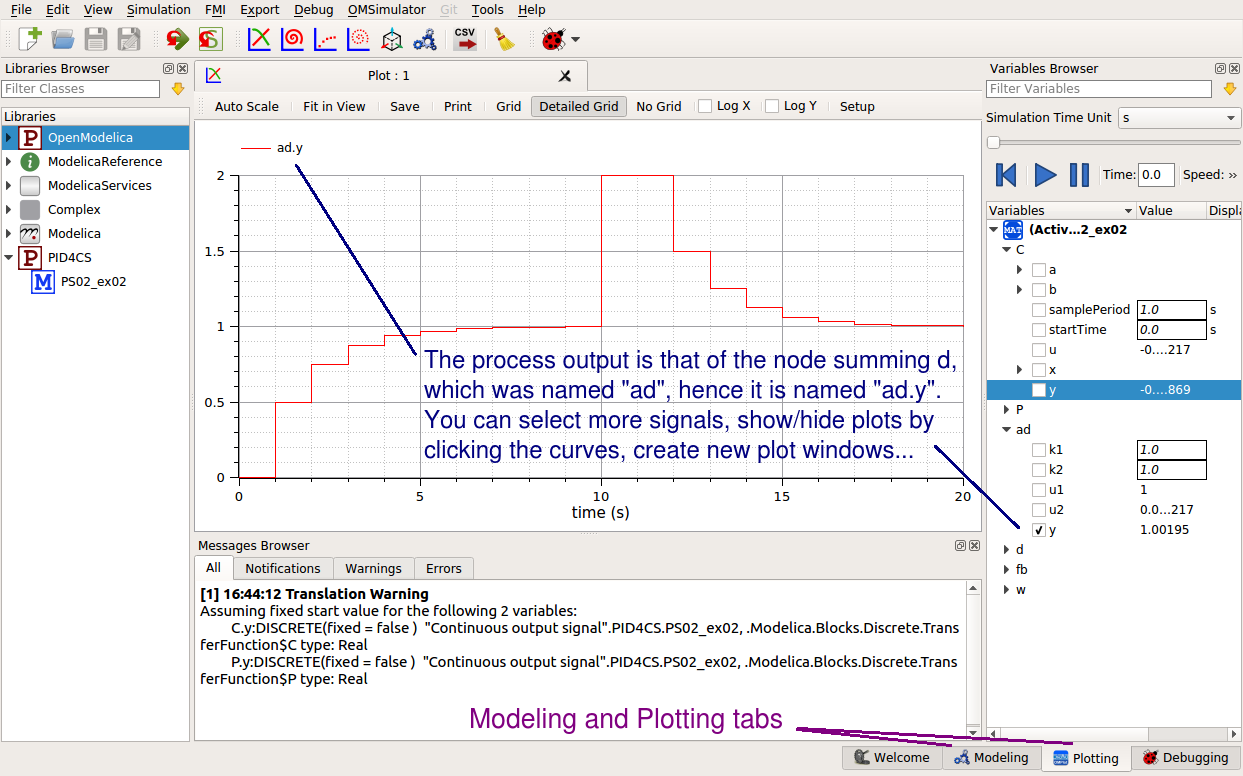
\includegraphics[width=0.60\columnwidth]{./Unit-05/img/PS02-ex02-fig03.png}
       \end{center}
 \end{itemize}
\end{frame}

\begin{frame}
\frametitleTC{Building a block diagram in Modelica}
\framesubtitleTC{and experimenting with direct synthesis}
\myPause
 \begin{itemize}[<+-| alert@+>]
 \item Please take some time at home to familiarise with OMEdit: it is quite intuitive\\
       and you can find plenty of tutorials online, many with videos. 
 \item For the moment, replicate for example the case with unstable hidden part:
       \begin{displaymath}
        \begin{array}{lcl}
         P(z)              = \frac{1}{\red{z-2}},\,
         G_{yw}^{\circ}(z) = \frac{0.2}{z-0.8} &
         \Rightarrow &
         C(z)              = \frac{0.2\red{(z-2)}}{z-1}.
        \end{array}
       \end{displaymath}
 \item Below is the plot of $y$ (\texttt{ad.y}) and $u$ (\texttt{C.y}) for $w=step(k)$ and $d=step(k-30)$.\\
       Apparently, something happens that $G_{yw}$ does not tell...
       \begin{center}
        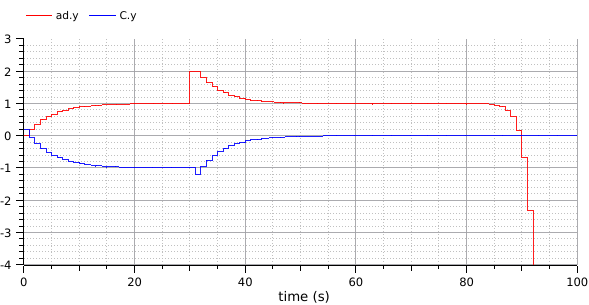
\includegraphics[width=0.50\columnwidth]{./Unit-05/img/PS02-ex02-fig04.png}
       \end{center}
 \end{itemize}
\end{frame}

